\documentclass[11pt,ngerman,a4paper,svgnames, oneside]{book}
\usepackage[utf8]{inputenc}
\usepackage[ngerman]{babel}
\usepackage[T1]{fontenc}
\usepackage{float}
\usepackage{graphicx}
\usepackage{todonotes}
\usepackage{tabularx}
\usepackage{nameref}
\usepackage{ltablex}
\usepackage{blindtext}
% Hyperref (sollte unbedingt vor geometry-Paket geladen werden)
% für Anzeige in Acrobat (pdfstartview)
\usepackage[bookmarks=false,
    pdfstartview=FitV,
    pdfhighlight={/I},
	colorlinks = true,
	linkcolor = blue,
	urlcolor  = blue,
	citecolor = blue,
    pdfborder={0 0 0},
    german]{hyperref}
\usepackage{inconsolata}
\usepackage{xcolor}
\usepackage{titling}
\usepackage{parskip}
\usepackage{cite}  
\usepackage{fancyhdr}
\usepackage{wrapfig}
\usepackage{pifont}
\usepackage{array}
\newcolumntype{P}[1]{>{\centering\arraybackslash}p{#1}}
\usepackage{pdflscape}
\usepackage{colortbl}
\usepackage{hhline} 
\usepackage{amssymb} 
\usepackage{animate}
\usepackage{amsmath}
\usepackage[export]{adjustbox}
\usepackage{subcaption}

\fancypagestyle{plain}{
	\fancyhf{}
	\chead{\leftmark }
	\renewcommand{\headrulewidth}{1pt}
	\renewcommand{\footrulewidth}{1pt}
	\rfoot{\small Seite \thepage}
}

\usepackage[left=2.5cm,right=2.5cm,top=3cm,bottom=4cm]{geometry}


\definecolor{pblue}{rgb}{0.13,0.13,1}
\definecolor{pgreen}{rgb}{0,0.5,0}
\definecolor{pred}{rgb}{0.9,0,0}
\definecolor{pgrey}{rgb}{0.46,0.45,0.48}
\definecolor{porange}{rgb}{1,0.4,0}
\colorlet{delim}{magenta!60!black}

\definecolor{lime}{rgb}{0.894,0.933,0.839}

\newcommand{\noncopynumber}[1]{
	\BeginAccSupp{method=escape,ActualText={}}
	#1
	\EndAccSupp{}
}

\usepackage{listings}
\lstset{language=Java,
	showspaces=false,
	showtabs=false,
	breaklines=true,
	showstringspaces=false,
	breakatwhitespace=true,
	commentstyle=\color{pgreen},
	keywordstyle=\color{pblue},
	stringstyle=\color{pred},
	basicstyle=\ttfamily,
	moredelim=[il][\textcolor{porange}]{\$\$},
	moredelim=[is][\textcolor{porange}]{\%\%}{\%\%},
	frame=single,
	numbers=left,
	numberstyle=\footnotesize,
	basicstyle=\ttfamily\footnotesize,
	xleftmargin=2.5em,
	xrightmargin=0.008\linewidth,
	rulecolor=\color{black},
	 postbreak=\mbox{\textcolor{red}{$\hookrightarrow$}\space},
	literate=
	*{\{}{{{\color{delim}{\{}}}}{1}
	{\}}{{{\color{delim}{\}}}}}{1}
	{[}{{{\color{delim}{[}}}}{1}
	{]}{{{\color{delim}{]}}}}{1}
}

\definecolor{lightgray}{rgb}{.9,.9,.9}
\definecolor{darkgray}{rgb}{.4,.4,.4}
\definecolor{purple}{rgb}{0.65, 0.12, 0.82}

\lstdefinelanguage{JavaScript}{
	keywords={typeof, new, true, false, catch, function, return, null, catch, switch, var, if, in, while, do, else, case, break},
	keywordstyle=\color{blue}\bfseries,
	ndkeywords={class, export, boolean, throw, implements, import, this, const},
	ndkeywordstyle=\color{darkgray}\bfseries,
	identifierstyle=\color{black},
	sensitive=false,
	comment=[l]{//},
	morecomment=[s]{/*}{*/},
	commentstyle=\color{pgreen}\ttfamily,
	stringstyle=\color{red}\ttfamily,
	morestring=[b]',
	morestring=[b]",
	moredelim=[is][\color{purple}]{|}{|},
	moredelim=[il][\textcolor{porange}]{\$\$},
	moredelim=[is][\textcolor{porange}]{\%\%}{\%\%}
}

\lstdefinelanguage{nginx}{
	keywords={upstream,server,listen,location,proxy\_pass},
	keywordstyle=\color{blue}\bfseries,
	ndkeywords={weight},
	ndkeywordstyle=\color{darkgray}\bfseries,
	identifierstyle=\color{black},
	sensitive=false,
	stringstyle=\color{red}\ttfamily,
	morestring=[b]',
	morestring=[b]"
}

\lstdefinelanguage{gradle}
{
	keywordstyle = {\color{blue}},
	keywordstyle = [2]{\color{purple}},
	keywords = {compile, testCompile, testCompileOnly},
	morekeywords = [2]{group, name, version},
	comment=[l]{//},
	commentstyle=\color{pgreen}\ttfamily,
}

\lstdefinestyle{Konsole}{
	frame=single,
	numbers=left,
	numberstyle=\small,
	breaklines=true,
	basicstyle=\small,
	xleftmargin=0.040\linewidth,
	xrightmargin=0.008\linewidth
}


\usepackage{caption}
\newcommand{\latex}{\LaTeX\xspace}

%DOCUMENT METADATA
\title{Computational Geometry and Virtual Reality - RunnAR}
\date{01. Januar 2019}
\author{Christian Schaf, Jannis Lindenberg, Vural Yilmaz}

\begin{document}
	\begin{titlepage}
		\begin{center}
			
\includegraphics[width=0.4\linewidth]{assets/logo.png} \\
			\huge\thetitle \\ \vspace{3cm}
			\Large\theauthor \\ \vspace{1cm}
			\thedate
		\end{center}
	\end{titlepage}
	\pagestyle{plain}
	\tableofcontents
	\listoffigures
	\chapter{Einleitung}
Im Rahmen des Moduls “Computational Geometry and Virtual Reality” wird eine Augmented Reality App entwickelt. Das Ziel dieses Projekts ist es, Objekte in einer durch AR erweiterten Realit\"at zu erkennen und in die Spielumgebung zu integrieren. Der Algorithmus-gesteuerte Spieler soll durch den A* Algorithmus m\"oglichst effizient den k\"urzesten Weg zwischen Start und Ziel nutzen, dabei variabel auf die sich st\"andig \"andernde Spielumgebung reagieren - wird ein neues Hindernis erkannt, muss der Weg des Computergesteuerten Spielers zum Ziel neu berechnet werden. 
Die Motivation hinter dieser Projektidee ist unter anderem im Rahmen dieses Projekts eine kleinen Einblick in die Entwicklung von Augmented Reality zu erhalten. Zusätzlich soll in Erfahrung gebracht werden, wie weit Augmented Reality Anwendungen mit der echten Umgebung interagieren können.

    \chapter{Grundlagen}
\label{sec:fundamentals}

    \chapter{Recherche}
\label{sec:recherche}


\section{A* Algorithmus}
Das Thema Wegfindung spielt in diesem Projekt eine wichtige Rolle. Der Computergegner soll einen Wegfindungs-Algorithmus benutzen, um den kürzesten Weg zum Ziel finden. Dabei soll die Wegfindung schnell und zuverlässig sein, auch wenn dynamisch ein oder mehrere Hindernisse auftauchen.

Zu den bekanntesten Algorithmen der Wegfindung gehören Dijkstra und A*.
-hier warum A*-
\section{Imagetargets}
\section{Objekterkennung}
Da die Objekterkennung einen großen Anteil des RunnAr Projekts ausmacht, wurde hierzu viel Recherche betrieben. Da die Objekte vom Benutzer in Echtzeit platziert und manipuliert werden können, wurde besonderes Augenmerk auf die Performanz der Implementierungsmöglichkeiten gerichtet.
\subsection{Tensorflow}
Tensorflow ist ein von Google entwickeltes Framework. Es wird oftmals in Programmen für maschinelles Lernen genutzt.  Implementiert ist es in Python und C++. Da Unity von Haus aus mit C Sharp Skripten arbeitet und keine alternative Sprache genutzt werden kann, muss für Unity das TensorFlowSharp Plugin genutzt werden. Dies stellt Wrapper zur Verfügung die den nativen C++ Code in C Sharp Code umwandeln. Auf Github finden sich einige Beispielprojekte, die den Fokus auf Objekterkennung setzen. Dies ermöglicht einen schnellen Einblick auf die Funktionalitäten von Tensorflow in Kombination mit Unity. Tensorflow ermöglicht es zwar durch trainierte Agenten eine große Variante an Objekten zu erkennen und zu klassifizieren, jedoch braucht dies seine Zeit. Die Kamera muss sich recht nah am Objekt befinden und Tensorflow verliert immer wieder den Fokus auf das Objekt. Zusätzlich ist die bounding Box, die sich um das Objekt dargestellt wird, recht grob. Bei diesem Ansatz fehlte für das Projekt also die Performanz und die Genauigkeit. Zusätzlich passte die Nähe die die Kamera zu dem Objekt haben musste nicht zu unserem Spielkonzept.

\subsection{OpenCv}
OpenCV ist eine freie Programmbibliothek zur Bildverarbeitung. Der Ansatz bei OpenCv wäre, dass Umrisse von auf dem Tisch platzierten Gegenständen erkennt werden sollten. Dies müsste jedoch auf einem hellen Untergrund geschehen, an dem sich die Objekte deutlich abheben. Der Vorteil gegenüber Tensorflow wäre hierbei, dass man keine trainierte Agenten bräuchte, die die Objekte zusätzlich klassifizieren würden. OpenCV hat jedoch den Nachteil, dass der Einsatz mit Unity kostenpflichtig ist. Die Kombination mit Unity ohne Kosten gestaltet sich als schwierig. Da Unity nur mit C Sharp Skripten arbeiten kann, müssten Wrapper erstellt werden, die die Kommunikation zu Unity ermöglichen würden. Fragwürdig wäre jedoch wie performant die Erkennung der Objekte mit OpenCv gewesen wäre.Viel Zeit und Aufwand hätten in die Entwicklung eines C++ Projekts mit OpenCv fließen müssen, bei der am Ende immer noch die Frage im Raum gewesen wäre, ob dies überhaupt flüssig in Unity laufen würde. Diesen Ansatz haben wir nach mehreren Tagen erfolgloser  Recherche und Implementierungsversuchen für ineffizient eingestuft. 

\subsection{Vuforia Object Recognition}
Vuforia verfügt nativ über Object Recognition. Hierbei müssen die Objekte, welche erkannt werden sollen, vorher durch eine kostenlose App für Android Geräte eingescannt werden. Hierfür kann man sich auf der Webseite von Vuforia eine Schablone ausdrucken, auf der man die zu scannenden Objekte platziert. Danach nutzt man die App und scannt die Objekte mit der Kamera auf dem mobilen Endgerät ein. Es wird virtuell ein Gitter um das platzierte Objekt dargestellt und die Bereiche die fertig gescannt wurden, werden grün markiert. Dies wiederholt man solange bis das Gitter komplett grün gefärbt ist.  Beim einscannen sollte man keine Objekte nehmen die zu klein sind, da diese recht lange brauchen um eingescannt zu werden. Zusätzlich ist die Erkennung kleiner Objekte nicht sehr effektiv, da Vuforia bei kleinen Objekte nicht ausreichend Vergleichspunkte hat um die Gegenstände zu erkennen. Die Performanz der eingescannten Objekte ist sehr gut, sodass die Einschränkung, dass nur eingescannte Objekte erkennt werden können, in Kauf genommen wurde. Auch die Erkennung auf weitere Entfernung ist gegeben. Nach dem Einscannen, können diese in eine Datenbank importiert werden und problemlos in Unity eingebunden werden. Mehr hierzu im Kapitel Umsetzung.

\section{Spielkonzept}

    \chapter{Konzept}
\label{sec:conzept}
In diesem Kapitel werden zum Einen die Funktionsanforderungen, die das Projekt am Tag der Abgabe erfüllen soll, aufgeführt. Nicht alle Vorhaben lassen sich in dem vorgegebenen Zeitraum umsetzten, sodass eine Liste aus Funktionsanforderungen gefertigt wird. Zum Anderen wird das Konzept für das Spiel RunnAR im Detail beschrieben.

\section{Definition von Funktionsanforderungen}
Bei der Abgabe des Projektes sollen folgende Anforderungen Teil des Funktionsumfang sein:
\begin{itemize}
\item Es soll einen festen Start- und Zielpunkt für die Berechnung des kürzesten Wegs vorhanden sein.
\item Eine algorithmus-gesteuerte Spielfigur soll den kürzesten Weg vom Start zum Ziel berechnen und ablaufen.
\item Es sollen auf dem Spielfeld platzierte Objekte als Hindernis anerkannt werden.
\item Die platzierten Hindernisse sollen von der Spielfigur umgangen werden und der kürzeste Weg soll neu berechnet werden.
\item Die Anwendung soll auf iOS und Android Geräten laufen.
\item Ein Timer soll die Zeit anzeigen, die der algorithmus-gesteuerte Spiel hat um zum Ziel  zu gelangen.
\item Der Spieler soll ein visuelles Feedback erhalten ob er gewonnen oder verloren hat.
\end{itemize}

\section{Spielkonzept}
Im Projekt RunnAR soll eine Spielfigur ein Hindernisfeld in einer vorgegebenen Zeit überwinden. Das Spielfeld befindet sich auf einer flachen Ebene und wird per Augmented Reality in die reale Welt projiziert. Die Hindernisse auf dem Spielfeld sind variabel und auch zur Spielzeit veränderbar. Der Spieler wird von einem Algorithmus gesteuert. Der Algorithmus steuert die Spielfigur in Richtung Ziel. Der Mensch als Gegenspieler versucht die Spielfigur, durch das Setzen von Hindernissen auf dem Spielfeld, daran zu hindern, das Ziel zu erreichen.\\
Die Spielidee basiert auf der Geschichte, dass ein Student den Studienalltag überleben muss. Hierbei werden die Hindernisse, den der Student ausweichen muss, durch bestimmte Gegenstände dargestellt. Bei den Gegenständen handelt es sich um Dinge, die einem Studenten den Studentenalltag erschweren. Ein solches Hindernis kann beispielsweise eine Straßenbahn sein, die stellvertretend für lange Fahrtzeiten zur Uni steht.\\
In Abbildung \ref{fig:conc_skizze} sind drei Beispielschritte eines Musterspielfelds abgebildet. Die Spielfigur (grüner Pullover), welche sich zu Beginn des Spiels am unteren Rand des Spielfelds befindet, muss den Hindernissen ausweichen. Hindernisse sind reale Objekte, die Im Spielfluss erkannt werden und so ein 3-dimensionales Hindernis für den Spieler darstellen. Der Start und das Ziel sind ebenfalls durch Muster gekennzeichnet. 

\begin{figure}[H]
    \centering
    \begin{subfigure}[b]{0.3\textwidth}
        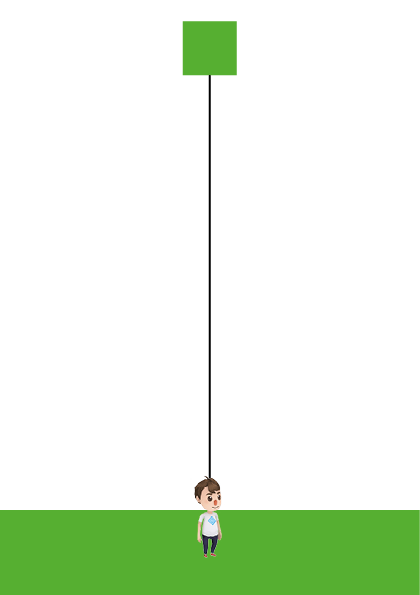
\includegraphics[width=\textwidth]{assets/skizze1.png}
        \caption{Projektskizze Teil 1}
        \label{fig:skizze1}
    \end{subfigure}
    ~
    \begin{subfigure}[b]{0.3\textwidth}
        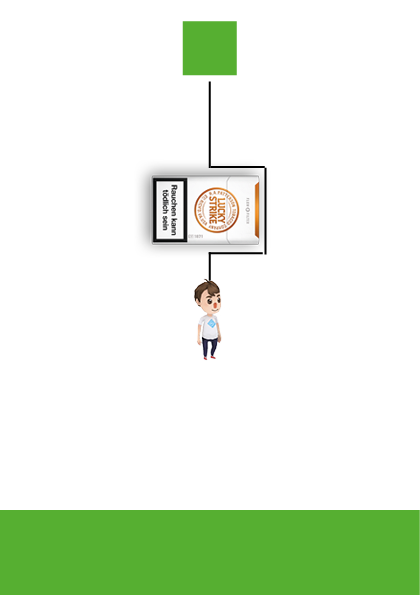
\includegraphics[width=\textwidth]{assets/skizze2.png}
        \caption{Projektskizze Teil 2}
        \label{fig:skizze2}
    \end{subfigure}
    ~
    \begin{subfigure}[b]{0.3\textwidth}
        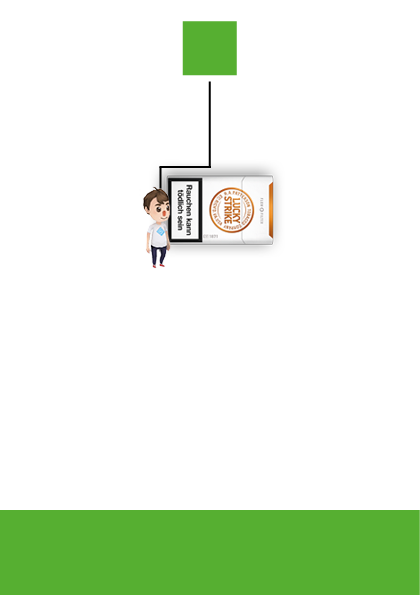
\includegraphics[width=\textwidth]{assets/skizze3.png}
        \caption{Projektskizze Teil 3}
        \label{fig:skizze3}
    \end{subfigure}
    \caption{Projektskizze}\label{fig:conc_skizze}
\end{figure}
    \chapter{Umsetzung}
\label{sec:Umsetzung}
\todo{Jannis}
\section{Implementierung des A* Algorithmus}
\label{sec:implementAStar}
\todo{Christian}
\section{ImageTargets}
Design der Images und Erkennung der Images
\section{Erkennung von Objekten}
Wie in Kapitel \ref{sec:vufObjRec} beschrieben müssen die eingescannten Objekte in eine Vuforia Datenbank importiert werden (siehe Abb. \ref{fig:vuforiaObjectDatabase}). Diese Datenbank wird im Vuforia Developer Portal zur Verfügung gestellt und ist mit wenigen Klicks eingerichtet. Diese Datenbank lässt sich für unterschiedliche Entwicklungsplattformen herunterladen. Unter anderem auch für die Unity IDE als package. Um die Objekte nun in der Unity Scene verwenden zu können, muss das Package per Import Package Funktion in Unity geladen werden.
\begin{figure}[h]
    \centering
    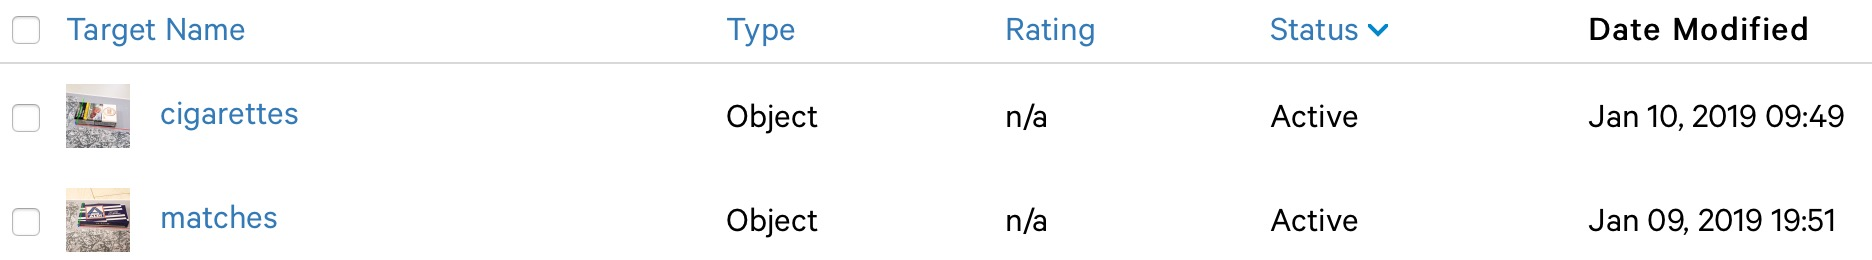
\includegraphics[width=\textwidth]{assets/vuforiaDataBase.jpeg}
    \caption{Vuforia Datenbank}\label{fig:vuforiaObjectDatabase}
\end{figure}\\
Vuforia bietet die Möglichkeit in Unity 3d Scan Objekte als Gameobjekt anzulegen. Bei dem angelegten Objekt kann nun die importierte Datenbank und das wiederzuerkennende Objekt ausgewählt werden. \\
In der Szene erscheint nun eine Bounding Box. Laut der Vuforia Dokumentation\cite{VufObjRec}  sollte die Bounding Box den Maßen des eingescannten Objektes entsprechen. Dies ist bei der Durchführung jedoch nicht der Fall gewesen. Die Objekte haben einen Nullpunkt. (siehe Abb. \ref{fig:matches}) Der Nullpunkt wird von der Schablone welche zum Einscannen genutzt wird, übernommen. Die Bounding Box bietet sich gut an, um Objekte auf dem eingescannten Objekt zu platzieren. Jedoch ist die Länge vom Nullpunkt bis zum Ende des Objektes nicht bekannt. Auch rechteckige Objekte werden durch eine quadratische Bounding Box dargestellt. Durch diesen Umstand kann keine präzise Bounding Box generiert werden, die das reale Objekt in der Scene widerspiegelt.\\
\begin{figure}[h]
    \centering
    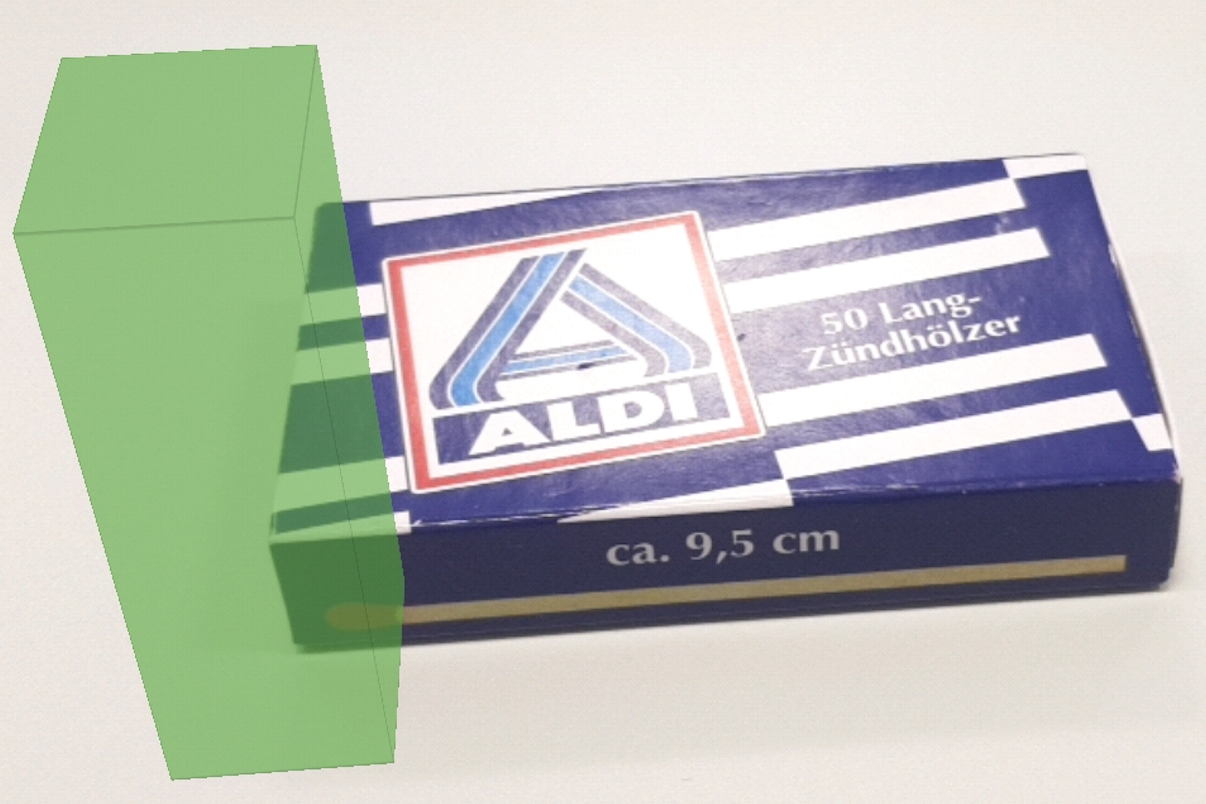
\includegraphics[width=0.5\linewidth]{assets/matches.png}
    \caption{Eingescanntes Objekt mit Nullpunkt}\label{fig:matches}
\end{figure}\\
Dem in der Scene befindlichen 3d Scan Game Object kann nun der \textit{unwalkable Layer} zugewiesen werden siehe \ref{sec:implementAStar} \nameref{sec:implementAStar}. Im Test reagierte der A* Algorithmus nicht auf die realen Objekte, da diese sich nicht auf der selben Ebene befinden wie das Spielfeld. Durch diesen Umstand haben wir den \textit{DefaultTrackableEventHandler} von Vuforia erweitert. Hierfür wurde ein eigenes Script implementiert, welches die eingescannten Objecte bei jedem Update auf die Position 0 der y-Achse transformiert. So wird sichergestellt, dass sich das reale Objekt und das Spielfeld auf der selben Ebene befinden. Das reale Objekt wurde daraufhin von den Nodes des A* Grids als unwalkable erkannt. \\
Um die Objekte in die Scene des Spielers zu integrieren muss sich die Kamera exakt über dem Spielfeld befinden. Eine Third Person Ansicht ist nicht möglich, da die erkannten Objekte von der Position der Kamera ausgehen. Steht die Kamera Beispielsweise auf xyz(0,-20, -20), erhält das gescannte Objekt ebenfalls diese Koordinaten. Wird das Objekt in der realen Welt bewegt, verändern sich die Koordinaten, allerdings ausgehend von der Kamera Position. Durch diesen Umstand muss die Kamera exakt in der Mitte des Spielfelds befinden, damit die realen Objekte ausgehend von diesem Punkt platziert werden können.

\section{UI}
Wie in Abbildung \ref{fig:uiElements} zu sehen ist, besteht das User Interface für die RunnAR Anwendung aus zwei unterschiedlichen Ansichten. Zum Einen ist in Abbildung \ref{fig:uiMenu}) das Startmenü zu sehen. Hierbei hat der Nutzer die Möglichkeit die Anwendung zu verlassen indem der Exit Button geklickt wird, oder das Spiel kann durch den Start Button gestartet werden. Zum Anderen besteht die Anwendung aus der Spielansicht (siehe Abbildung \ref{fig:uiGame}). Die Spielansicht beinhaltet einen Replay Button, einen Timer sowie den Spieler und alle Interaktionselemente für den Spieler. Durch den Replay Button lässt sich der derzeitige Spielstand zurücksetzen und von Neuem beginnen. Der Timer läuft von 90 Sekunden bis 0. Ist die Zeit abgelaufen ist die Spielrunde beendet. Das UI der Anwendung befindet sich in einem prototypischen Zustand, der eine einfache Bedienung ermöglicht.

\begin{figure}[H]
    \centering
    \begin{subfigure}[b]{0.3\textwidth}
        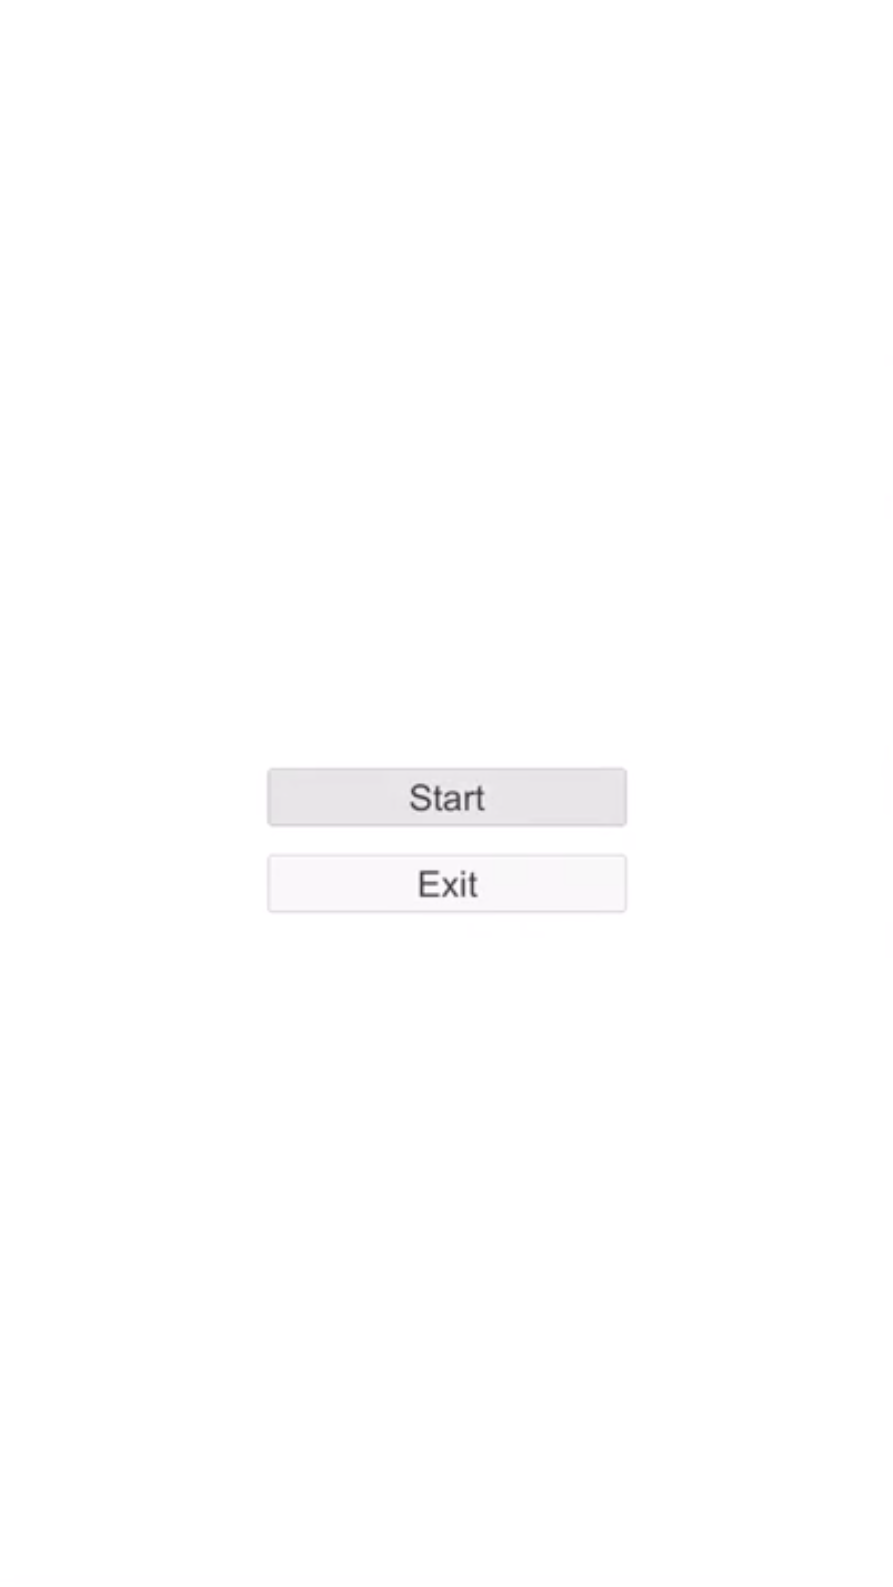
\includegraphics[width=\textwidth]{assets/uiMenu}
        \caption{UI Menüansicht}
        \label{fig:uiMenu}
    \end{subfigure}
    ~
    \begin{subfigure}[b]{0.3\textwidth}
        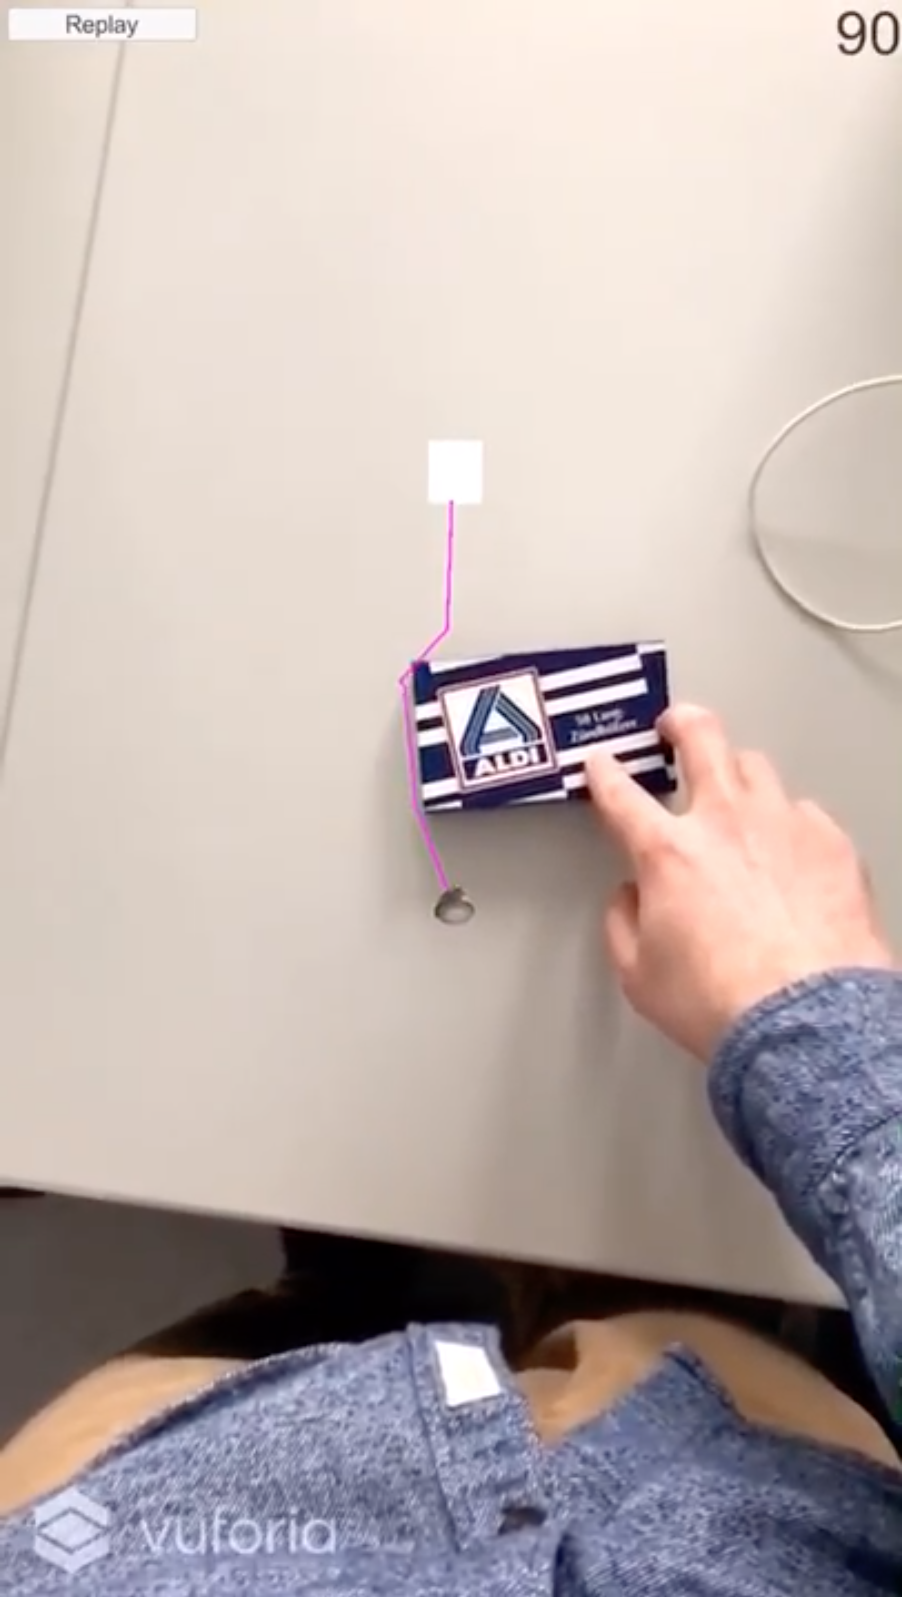
\includegraphics[width=\textwidth]{assets/uiGame}
        \caption{UI Spielansicht}
        \label{fig:uiGame}
    \end{subfigure}
    \caption{User Interface Elemente}\label{fig:uiElements}
\end{figure}


    \chapter{Zusammenfassung und Fazit}

Die Interaktion von AR-Objekten und echten Objekten gestaltet sich schwierig. Die Performanz der Vuforia Objekt Recognition ist gut, jedoch ist das Vuforia SDK unausgereift. Das Fehlen einer präzisen Bounding Box erschwert die Berechnung der Wegfindung, da die Größe des Objekts im Spielfeld nicht klar ersichtlich ist. Zusätzlich ist Unity sehr konfigurationslastig, was auch bei kleinen Änderungen in der Konfiguration große Auswirkungen auf die Spielszene haben kann.  Mehrere Leute können nicht gleichzeitig in einer Szene arbeiten, da eine Szene aus einer Datei besteht, die sich schwierig mergen lässt. Dies erschwerte die Teamarbeit per Versionsverwaltung. Der Objekterkennungsansatz ist unserem Projekt ist sehr experimentell. Es war uns nicht möglich einen ähnlichen Ansatz für die Nutzung der Objekterkennung in einer AR Anwendung zu finden. Dies streut den Verdacht, dass AR zwar gut dafür ist AR-Objekte in die reale Welt zu platzieren, jedoch der Use-Case den wir für unser Projekt gewählt haben momentan nicht möglich ist. Dieses Projekt hatte ein großes Forschungsdelta, da wir uns gut in Unity einarbeiten konnten und viel Zeit in die Recherche und die verschiedenen Ansätze der Objekterkennung investiert haben. 


Als Ausblick könnte man in RunnAr dynamische Ziele einbauen, die durch ImageTargets repräsentiert werden. Zusätzlich könnte das vorbereite Skript für die schießende Elemente eingebaut werden, dessen Projektilen der Algorithmus zusätzlich ausweichen müsste. Dies könnte auch den Spielfluss verbessern. Der Kamerawinkel könnte angepasst werden, um die Vogelperspektive in eine isometrische Ansicht zu ändern. So hätte man ein besseren Ansicht auf die Spielumgebung. Dazu müsste man jedoch den Versuch unternehmen, die Spielfigur auf der gleichen Ebene wie die gesetzten Objekte zu platzieren. Als Ansatz würde sich hier eine Ground Detection anbieten, die erweitert werden müsste um nicht nur Objekte zu platzieren, sondern auch die Spielfigur auf dem Tisch weitgehend realistisch in Bewegung darstellt.
    \chapter{Anhang}
\label{sec:anhang}

    \nocite{*}
    \bibliographystyle{IEEEtran}
	\bibliography{library}
\end{document}
